\documentclass[11pt,twoside]{article}
\usepackage{amsmath}
\usepackage{amssymb}
\usepackage{amsthm}
\usepackage{amsfonts}
\usepackage{microtype}
\usepackage{hyperref}
\usepackage{graphicx}
\usepackage{tikz}
\usepackage{mathrsfs}

\newtheorem{theorem}{Theorem}
\newtheorem{lemma}{Lemma}
\newtheorem{proposition}{Proposition}
\newtheorem{corollary}{Corollary}
\newtheorem{definition}{Definition}
\newtheorem{conjecture}{Conjecture}
\newtheorem{remark}{Remark}

\title{\textbf{Spectral Methods in Data Compression and Geometric Encoding: \\
Block Entropy, Information Conservation, and Generalized Surfaces of Revolution}}
\author{\textbf{Padraic} \\ \textit{Independent Researcher}}
\date{\today}

\begin{document}

\maketitle

\begin{abstract}
We present three interconnected investigations at the intersection of information theory, signal processing, and differential geometry. First, we formalize the observation that grouping a binary string into blocks of size $n$ and computing the resulting $n$-gram entropy reveals a spectral structure: the block size that minimizes the per-bit entropy corresponds to the dominant period of the string, recoverable in $\mathcal{O}(N \log N)$ time via the Fast Fourier Transform. Second, we provide a rigorous analysis of why encoding binary data onto continuous curves---whether sinusoidal trajectories or high-degree polynomials---and applying Fourier series compression necessarily fails, tracing the obstruction to a fundamental conservation of degrees of freedom and the floating-point inflation penalty. Third, we develop the theory of generalized surfaces of revolution, wherein a target curve is rotated about a curved axis parameterized by the Frenet--Serret frame expressed through unit quaternions in $\mathbb{H}$, establishing a structural connection to the $\operatorname{SU}(2)$ sandwich operator of quantum mechanics. We show that taking the winding number to infinity yields a spiral space-filling path that reduces the dimensionality of the surface from $\mathbb{R}^3$ to a single $1$-dimensional signal amenable to classical spectral compression.
\end{abstract}

%=============================================================================
\section{Introduction}
%=============================================================================

The central thread unifying the three investigations in this paper is the interplay between \emph{discrete information} and \emph{continuous representation}. Shannon's source coding theorem \cite{CoverThomas} establishes a hard lower bound on the expected codeword length for lossless compression. Yet the bound applies to a specific probability model, and by changing the model---grouping symbols into blocks, shifting alignment, or transforming the representation space---one can appear to violate the bound while in fact operating under a different (and tighter) entropy measure.

This observation motivates Part~I, where we formalize the block entropy framework and show that the FFT provides an efficient mechanism for finding the natural ``fundamental frequency'' of a binary string. Part~II examines the converse question: can we \emph{gain} compressibility by embedding discrete data into a continuous domain? We show rigorously that the answer is no, due to an information-theoretic conservation law. Part~III departs from compression to develop a geometric framework---generalized surfaces of revolution around curved axes---that unexpectedly reconnects to compression through a spiral dimensional reduction that \emph{does} produce a compressible continuous signal from a 3D surface.

%=============================================================================
\part*{I. Block Entropy and FFT-Based Compression}
%=============================================================================

\section{First-Order Shannon Entropy and Its Limitations}

Let $\mathbf{b} = (b_1, b_2, \dots, b_N)$ be a binary string of length $N$, with $b_i \in \{0, 1\}$. The first-order Shannon entropy of $\mathbf{b}$ is
\begin{equation}
	H_1(\mathbf{b}) = -p_0 \log_2 p_0 - p_1 \log_2 p_1,
\end{equation}
where $p_0$ and $p_1$ are the empirical frequencies of $0$ and $1$ in $\mathbf{b}$. This quantity assumes the source is \emph{memoryless}: the probability of each bit is independent of all others.

If $\mathbf{b}$ possesses any sequential structure---repeating patterns, Markov dependencies, or periodic motifs---$H_1$ completely fails to capture it. A string such as $\mathbf{b} = 01010101\dots$ has $p_0 = p_1 = 1/2$ and thus $H_1 = 1$ bit, yet it is trivially compressible because the entire string is determined by a single bit and a period.

\section{Block Entropy and Symbol Extension}

\begin{definition}[Block Entropy]
	For a positive integer $n$ dividing $N$, partition $\mathbf{b}$ into $N/n$ consecutive non-overlapping blocks of $n$ bits. Each block is interpreted as a symbol from the alphabet $\Sigma_n = \{0, 1\}^n$ of cardinality $2^n$. Let $p_\sigma^{(n)}$ denote the empirical frequency of symbol $\sigma \in \Sigma_n$. The \emph{$n$-gram block entropy} is
	\begin{equation}
		H_n(\mathbf{b}) = -\sum_{\sigma \in \Sigma_n} p_\sigma^{(n)} \log_2 p_\sigma^{(n)}.
	\end{equation}
	The \emph{per-bit block entropy} is $h_n(\mathbf{b}) = H_n(\mathbf{b}) / n$.
\end{definition}

\begin{proposition}[Monotonicity of Per-Bit Block Entropy]
	For any stationary source, the per-bit block entropy is non-increasing:
	\begin{equation}
		h_n(\mathbf{b}) \leq h_{n-1}(\mathbf{b}) \leq \cdots \leq h_1(\mathbf{b}) = H_1(\mathbf{b}).
	\end{equation}
	Equality holds throughout if and only if the source is memoryless.
\end{proposition}

\begin{proof}
	By the chain rule of entropy, the joint entropy of a block of length $n$ is:
	\begin{equation}
		H_n(\mathbf{b}) = H(b_1, \dots, b_n) = \sum_{i=1}^n H(b_i \mid b_1, \dots, b_{i-1}).
	\end{equation}
	For a stationary source, conditioning reduces entropy, which means the conditional entropies are monotonically non-increasing:
	\begin{equation}
		H(b_i \mid b_1, \dots, b_{i-1}) \leq H(b_{i-1} \mid b_1, \dots, b_{i-2}).
	\end{equation}
	Thus, the sequence of conditional terms is bounded above by the previous terms, making the running average $h_n(\mathbf{b}) = \frac{1}{n} \sum_{i=1}^n H(b_i \mid b_1, \dots, b_{i-1})$ monotonically non-increasing as $n$ increases. Equality $h_n = H_1$ holds if and only if there is no dependence between bits, which is the definition of a memoryless source.
\end{proof}

\begin{figure}[htbp]
	\centering
	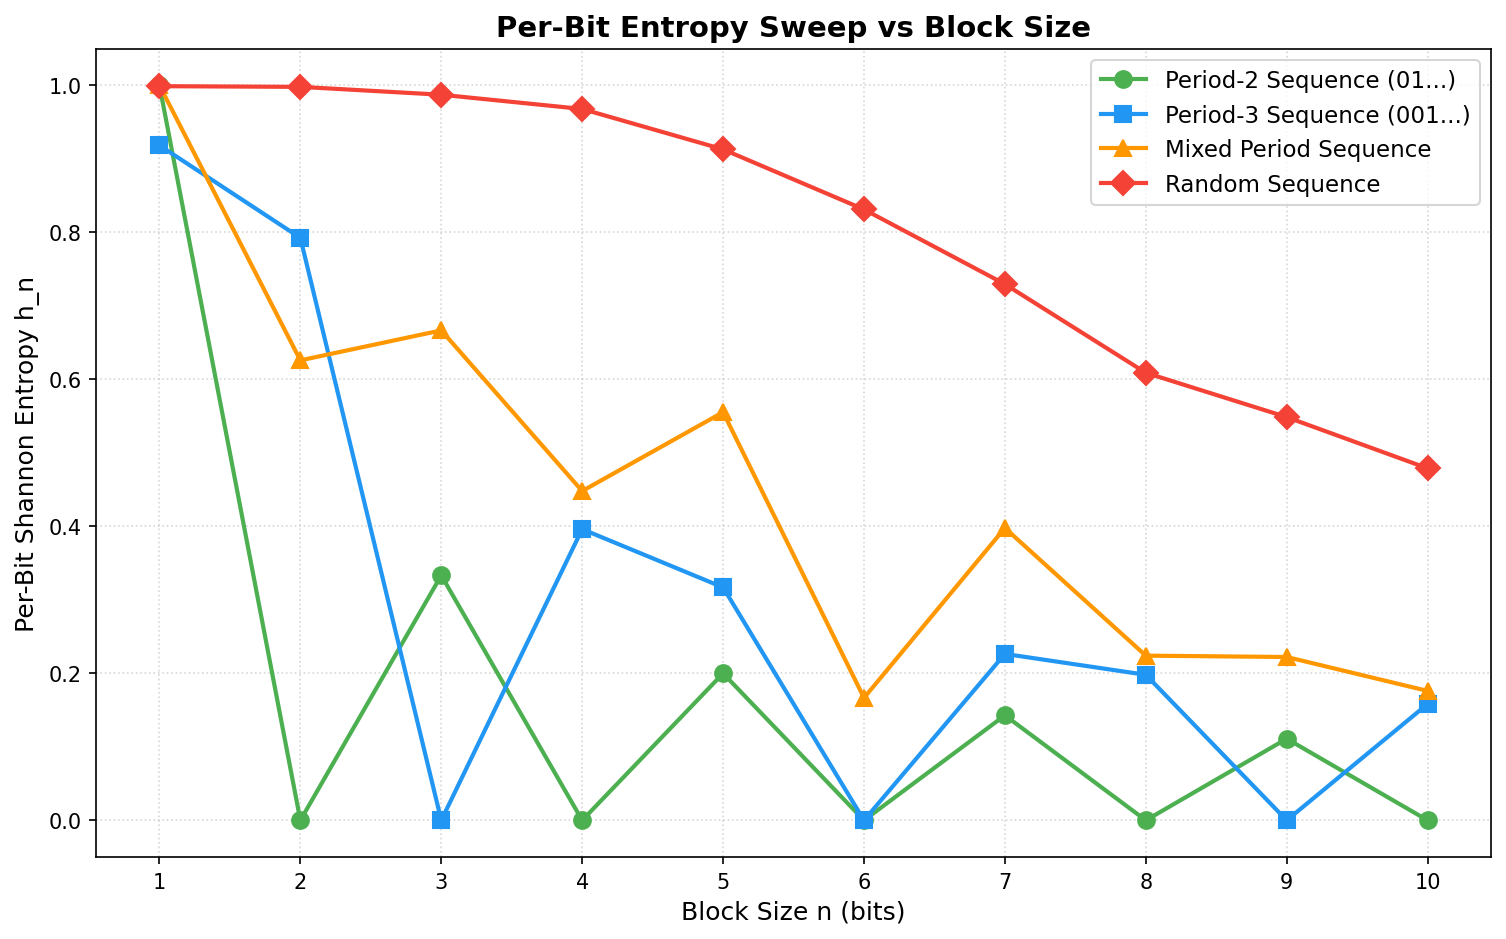
\includegraphics[width=0.8\textwidth]{figures/block_entropy_sweep.png}
	\caption{Per-bit Shannon entropy $h_n$ as a function of block size $n$ for four distinct test sequences. Periodic sequences exhibit sharp local minima at integer multiples of their fundamental period, whereas the random sequence remains flat near the theoretical maximum of $1.0$ bit.}
	\label{fig:block_entropy_sweep}
\end{figure}

\begin{remark}
	By sweeping $n$ over candidate block sizes and evaluating $h_n$, one searches for the \emph{natural word length} of the data---the block size at which the per-bit entropy is minimized. If the string has an underlying period of $T$ bits, then $n = T$ (or a multiple thereof) will yield a maximally skewed symbol distribution and thus the lowest $h_n$.
\end{remark}

\subsection{Cyclic Shifts and Padding}

When $n \nmid N$, we extend $\mathbf{b}$ by cyclic repetition (looping the string on itself) and pad with zeros to the nearest multiple of $n$. Let $s \in \{0, 1, \dots, n-1\}$ denote a bit-level shift applied before blocking. The per-bit entropy becomes a function of both block size and shift:
\begin{equation}
	h_{n,s}(\mathbf{b}) = \frac{1}{n} H\bigl(\text{BlockPartition}(\text{Shift}_s(\mathbf{b}), n)\bigr).
\end{equation}
The optimal compression parameters are
\begin{equation}
	(n^*, s^*) = \operatorname*{arg\,min}_{n, s} \; h_{n,s}(\mathbf{b}).
\end{equation}

\subsection{Metadata Overhead}

To decompress the string, the decoder requires: the chosen block size $n^*$, the shift $s^*$, and the Huffman dictionary for the $n^*$-bit alphabet. For short strings (say $N < 100$), this metadata can dominate the total compressed size. However, the overhead is $\mathcal{O}(\log N + 2^{n^*})$ bits, which is amortized as $N \to \infty$.

\section{The FFT as a Period Detector}

Rather than brute-force search over all $(n, s)$ pairs, we exploit the duality between periodicity detection and spectral analysis.

\subsection{Signal Conversion}

Map the binary string to a zero-mean real signal:
\begin{equation}
	x_i = 2b_i - 1, \qquad x_i \in \{-1, +1\}.
\end{equation}

\subsection{Autocorrelation via the Wiener--Khinchin Theorem}

The autocorrelation $R(\tau) = \sum_{i} x_i \, x_{i+\tau}$ measures how well the signal matches a time-shifted copy of itself. By the Wiener--Khinchin theorem, $R(\tau)$ is the inverse Fourier transform of the power spectral density:
\begin{equation}
	R(\tau) = \mathcal{F}^{-1}\!\left[\, |\hat{X}(f)|^2 \,\right](\tau),
\end{equation}
where $\hat{X}(f) = \mathcal{F}[x](f)$ is the discrete Fourier transform.

\begin{theorem}[FFT Period Detection]
	Let $\hat{X}(f)$ be the DFT of the signal $(x_1, \dots, x_N)$, and let $f_{\max}$ be the frequency bin maximizing the power spectral density $|\hat{X}(f)|^2$ (excluding the DC component $f = 0$). Then the dominant period of the string is
	\begin{equation}
		T = \frac{N}{f_{\max}},
	\end{equation}
	and the optimal block size is $n^* = \operatorname{round}(T)$.
\end{theorem}

\subsection{Phase Extraction for Optimal Shift}

The FFT yields complex coefficients $\hat{X}(f) = A(f) e^{i\phi(f)}$. The phase angle $\phi(f_{\max})$ at the dominant frequency encodes the alignment of the periodic pattern relative to the start of the string:
\begin{equation}
	s^* = \operatorname{round}\!\left(\frac{\phi(f_{\max})}{2\pi} \cdot T\right) \bmod T.
\end{equation}

This extracts both optimal parameters in $\mathcal{O}(N \log N)$ time, compared to $\mathcal{O}(N \cdot T_{\max}^2)$ for brute-force search.

\subsection{The Goertzel Optimization}

When the candidate block sizes are restricted to powers of $2$ (i.e., $n \in \{2, 4, 8, 16, \dots\}$), one need only evaluate the power spectrum at $\mathcal{O}(\log N)$ specific frequency bins. The Goertzel algorithm computes the DFT at a single target frequency in $\mathcal{O}(N)$ time, yielding a total complexity of $\mathcal{O}(N \log N)$ for the restricted search.

\begin{figure}[htbp]
	\centering
	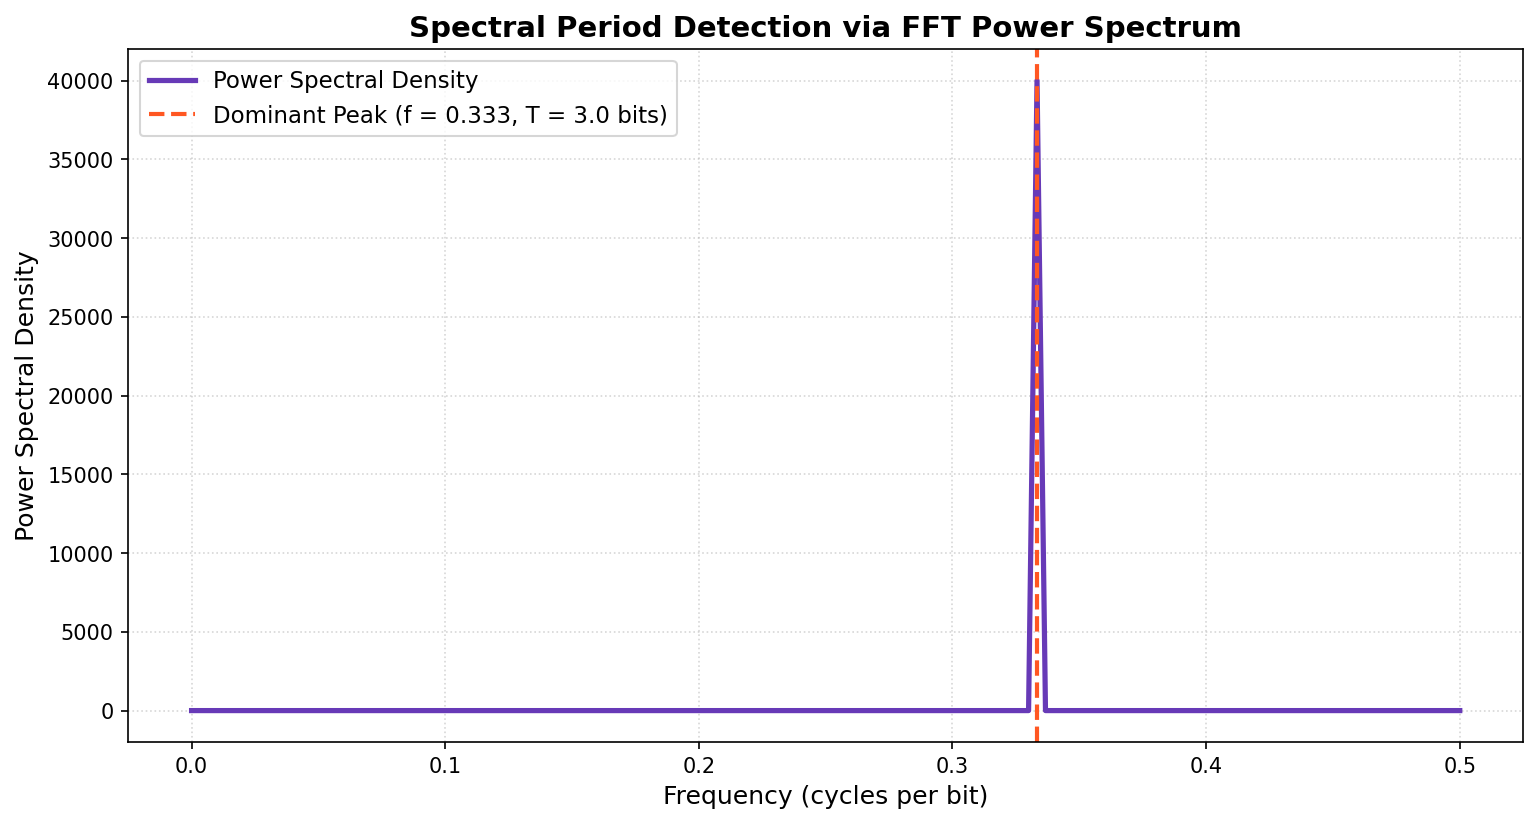
\includegraphics[width=0.8\textwidth]{figures/fft_period_detection.png}
	\caption{Discrete Fourier Transform power spectrum (PSD) of a binary sequence of period $T = 3$. The prominent peak at $f = 0.333$ cycles/bit corresponds exactly to the fundamental period, allowing rapid structural period identification in $\mathcal{O}(N \log N)$ operations.}
	\label{fig:fft_period_detection}
\end{figure}

%=============================================================================
\part*{II. Information Conservation Under Domain Transforms}
%=============================================================================

\section{Motivation: Encoding Binary Data on Continuous Curves}

A natural question arises: if the Fourier transform can compress audio signals and images by discarding negligible high-frequency coefficients, can we embed a binary string into a continuous function and compress it via Fourier series?

We examine two specific encoding schemes and prove that both necessarily \emph{expand} the data rather than compress it.

\section{Scheme A: Slope-Modulated Sinusoidal Encoding}

\subsection{Construction}

Given $N$ bits, partition them into $4$ chunks of $N/4$ bits, one per quadrant of a sinusoidal template. Consider the first quadrant: we construct a piecewise-linear path from $(0, 0)$ to $(\pi/2, 1)$ using $N/4$ discrete steps. At each step $i$:
\begin{itemize}
	\item If $b_i = b_{i-1}$ (no transition), the slope remains unchanged.
	\item If $b_i \neq b_{i-1}$ (transition), the slope decreases by $\frac{4}{N}$.
\end{itemize}
Starting from maximal slope at the origin, the boundary conditions are enforced so the curve passes through $(\pi/2, 1)$, $(\pi, 0)$, $(3\pi/2, -1)$, and $(2\pi, 0)$---matching $\sin(x)$ at multiples of $\pi/2$.

\begin{remark}
	A uniform string (all identical bits) produces a straight line from $(0,0)$ to $(\pi/2, 1)$. A maximally alternating string produces a piecewise-linear approximation of $\sin(x)$.
\end{remark}

\subsection{Why Fourier Compression Fails}
The resulting piecewise-linear curve has $N/4$ ``knuckle points'' where the slope changes. Each knuckle is a discontinuity in the first derivative.

\begin{theorem}[Degrees of Freedom Preservation]
	Let $y(x)$ be a continuous piecewise-linear curve on $[0, 2\pi]$ with $K$ slope discontinuities representing a binary sequence. To reconstruct $y(x)$ losslessly from its Fourier series coefficients, at least $K$ non-zero coefficients are required.
\end{theorem}

\begin{proof}
	A continuous piecewise-linear curve with $K$ knots is uniquely parameterized by the $K$ slopes $\{s_i\}_{i=1}^K$ of its segments (and one initial value $y(0)$). Thus, the space of such curves is a linear subspace $V \subset L^2([0, 2\pi])$ of dimension $K+1$.
	
	The Fourier transform $\mathcal{F}: L^2([0, 2\pi]) \to \ell^2(\mathbb{Z})$ is a unitary linear operator. By the rank-nullity theorem, the image of $V$ under $\mathcal{F}$ must also be a linear subspace of dimension $K+1$. Consequently, any basis of the image space requires at least $K+1$ coordinates. If we truncate the Fourier series to fewer than $K$ coefficients, the projection operator has a non-trivial kernel, meaning multiple distinct binary strings will map to the same truncated Fourier representation, violating injectivity (lossless reconstruction).
\end{proof}

\begin{figure}[htbp]
	\centering
	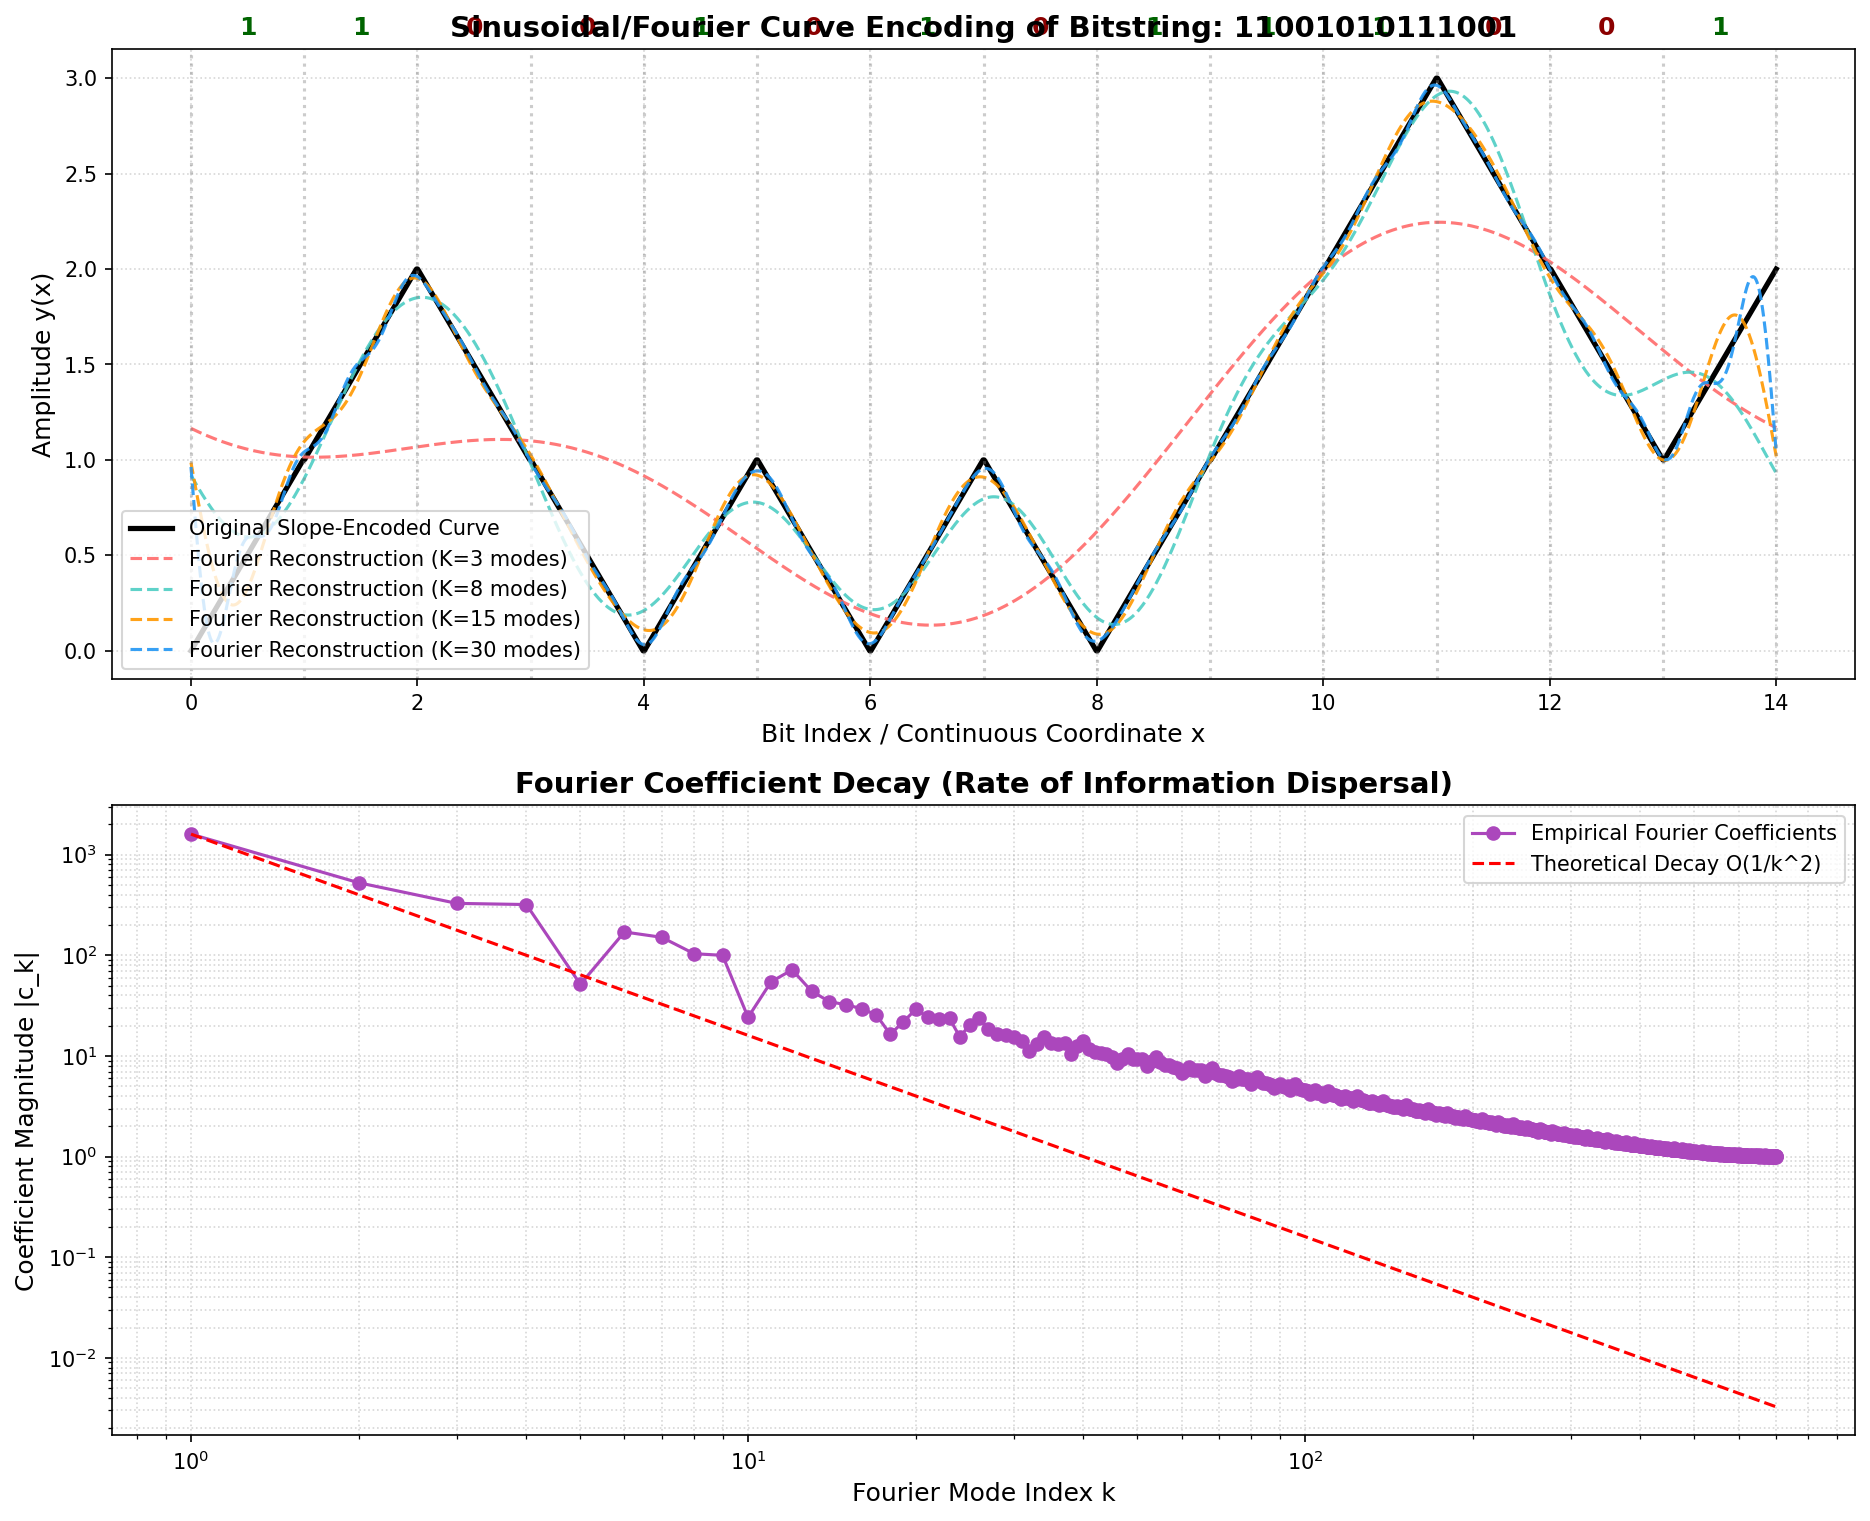
\includegraphics[width=0.95\textwidth]{figures/piecewise_linear_encoding.png}
	\caption{Slope-modulated piecewise-linear encoding of a binary string (top panel) and the corresponding Fourier coefficient decay (bottom panel). To resolve the $K$ knuckle points without loss, we require at least $K$ modes. The coefficients decay as $\mathcal{O}(1/k^2)$, demonstrating that high frequencies cannot be discarded without smoothing the corners and losing the underlying bits.}
	\label{fig:piecewise_linear_encoding}
\end{figure}

\section{Scheme B: Polynomial Interpolation Followed by Fourier Analysis}

\subsection{Construction}
Instead of connecting the slope-determined points with line segments, fit a smooth polynomial through all $K = N/4$ data points. This eliminates derivative discontinuities.

\subsection{Runge's Phenomenon and Degree Explosion}
A polynomial passing through $K$ arbitrary points has degree at most $K - 1$, requiring $K$ coefficients $(a_0, a_1, \dots, a_{K-1})$. The polynomial oscillates violently between data points (Runge's phenomenon), generating massive high-frequency energy in the Fourier domain.

\begin{theorem}[Information Conservation Law]
	Let $\mathbf{b} \in \{0,1\}^N$ be a binary string and let $\Phi: \{0,1\}^N \to \mathbb{R}^M$ be any injective (lossless) map into a space of real-valued parameters. If each real parameter is represented with a bit-width of $B$ bits (e.g., $B = 32$ for single-precision floats or $B = 64$ for double-precision), then:
	\begin{equation}
		M \cdot B \geq N.
	\end{equation}
\end{theorem}

\begin{proof}
	By definition of injectivity, the cardinality of the image must satisfy $|\Phi(\{0,1\}^N)| = 2^N$. The parameters live in a discrete machine representation space $\mathcal{M}^M$ where $|\mathcal{M}| = 2^B$. The total number of representable states is $(2^B)^M = 2^{M \cdot B}$. For the mapping to be injective, the number of target states must be at least the number of source states:
	\begin{equation}
		2^{M \cdot B} \geq 2^N \implies M \cdot B \geq N. \qedhere
	\end{equation}
\end{proof}

\begin{corollary}[Sinusoidal Inflation Penalty]
	If we encode $N$ bits onto a continuous curve using $M = N/4$ coefficients stored as 32-bit floats, the required storage is $32 M = 8 N$ bits. This represents an $8\times$ expansion (inflation penalty) of the data representation.
\end{corollary}

\begin{remark}[Connection to Telecommunications]
	While Fourier-based encoding fails as a \emph{compressor}, it is precisely the mathematical framework used for modern wireless data \emph{transmission}. OFDM (Orthogonal Frequency-Division Multiplexing) and QAM (Quadrature Amplitude Modulation) map binary bits onto the amplitudes and phases of sinusoidal subcarriers---not to compress data, but to transmit it efficiently over analog channels.
\end{remark}

%=============================================================================
\part*{III. Generalized Surfaces of Revolution via Quaternionic Frames}
%=============================================================================

\section{Classical Surfaces of Revolution}

A classical surface of revolution is generated by rotating a \emph{target curve} $C(s)$ about a straight-line axis. If $C(s) = (f(s), 0, s)$ and the axis is the $z$-axis, the resulting surface is parameterized by
\begin{equation}
	\mathbf{r}(s, \theta) = \bigl(f(s)\cos\theta, \; f(s)\sin\theta, \; s\bigr), \qquad \theta \in [0, 2\pi).
\end{equation}

We seek to generalize this construction to allow rotation about a \emph{curved} axis.

\section{The Curved Axis and Moving Frame}

\begin{definition}[Axis Curve]
	Let $\gamma: [a, b] \to \mathbb{R}^3$ be a smooth, regular curve parameterized by arc length $s$, with curvature $\kappa(s) > 0$ and torsion $\tau(s)$.
\end{definition}

At each point $\gamma(s)$, we define the Frenet--Serret moving frame \cite{DoCarmo} $\{\mathbf{T}(s), \mathbf{N}(s), \mathbf{B}(s)\}$, satisfying
\begin{equation}
	\frac{d}{ds}
	\begin{pmatrix} \mathbf{T} \\ \mathbf{N} \\ \mathbf{B} \end{pmatrix}
	=
	\begin{pmatrix} 0 & \kappa & 0 \\ -\kappa & 0 & \tau \\ 0 & -\tau & 0 \end{pmatrix}
	\begin{pmatrix} \mathbf{T} \\ \mathbf{N} \\ \mathbf{B} \end{pmatrix}.
\end{equation}

\begin{definition}[Target Curve and Radius Function]
	Let $C$ be a second curve. At each $s \in [a, b]$, the normal line from $\gamma(s)$ along $\mathbf{N}(s)$ intersects $C$ at a point whose distance from $\gamma(s)$ defines the \emph{radius function} $r(s)$.
\end{definition}

\begin{definition}[Non-Degeneracy Condition]
	The construction is non-degenerate when the maximum radius does not exceed the minimum radius of curvature of the axis:
	\begin{equation}
		\max_{s \in [a,b]} r(s) < \min_{s \in [a,b]} \frac{1}{\kappa(s)}.
	\end{equation}
	This prevents the coordinate system from folding (self-intersecting normal planes).
\end{definition}

\begin{proposition}[Tubular Neighborhood and Jacobian Non-Vanishing]
	The non-degeneracy condition is necessary and sufficient for the map $\mathbf{r}(s, \theta)$ to be a local diffeomorphism onto its image.
\end{proposition}

\begin{proof}
	Define the coordinate map $\Phi(s, u, v) = \gamma(s) + u \mathbf{N}(s) + v \mathbf{B}(s)$ on a domain where $u^2 + v^2 \leq r(s)^2$. The columns of the Jacobian matrix $J = [\partial_s \Phi, \partial_u \Phi, \partial_v \Phi]$ are:
	\begin{align}
		\partial_s \Phi &= \gamma'(s) + u \mathbf{N}'(s) + v \mathbf{B}'(s) = (1 - u \kappa(s)) \mathbf{T}(s) - v \tau(s) \mathbf{N}(s) + u \tau(s) \mathbf{B}(s), \\
		\partial_u \Phi &= \mathbf{N}(s), \\
		\partial_v \Phi &= \mathbf{B}(s).
	\end{align}
	The volume element (Jacobian determinant) is the triple product of these columns:
	\begin{equation}
		\det J = \partial_s \Phi \cdot (\partial_u \Phi \times \partial_v \Phi) = \partial_s \Phi \cdot \mathbf{T}(s) = 1 - u \kappa(s).
	\end{equation}
	For the map to be a local diffeomorphism, we require $\det J \neq 0$. Since $u = \rho \cos\theta$ for $0 \leq \rho \leq r(s)$, the range of $u$ is $[-r(s), r(s)]$. The condition $1 - u \kappa(s) > 0$ holds everywhere if and only if $r(s) < 1/\kappa(s)$ for all $s \in [a, b]$, which is the non-degeneracy condition.
\end{proof}

\section{Generalized Surface of Revolution}

The generalized surface is parameterized by
\begin{equation}
	\mathbf{r}(s, \theta) = \gamma(s) + r(s)\bigl[\cos\theta \; \mathbf{N}(s) + \sin\theta \; \mathbf{B}(s)\bigr], \qquad \theta \in [0, 2\pi).
\end{equation}

When $\gamma$ is a straight line ($\kappa = 0$), $\mathbf{N}$ and $\mathbf{B}$ are constant and this reduces to the classical surface of revolution. For a curved axis, the Frenet frame rotates along the path, ``twisting'' the surface according to the torsion $\tau(s)$.

\begin{figure}[htbp]
	\centering
	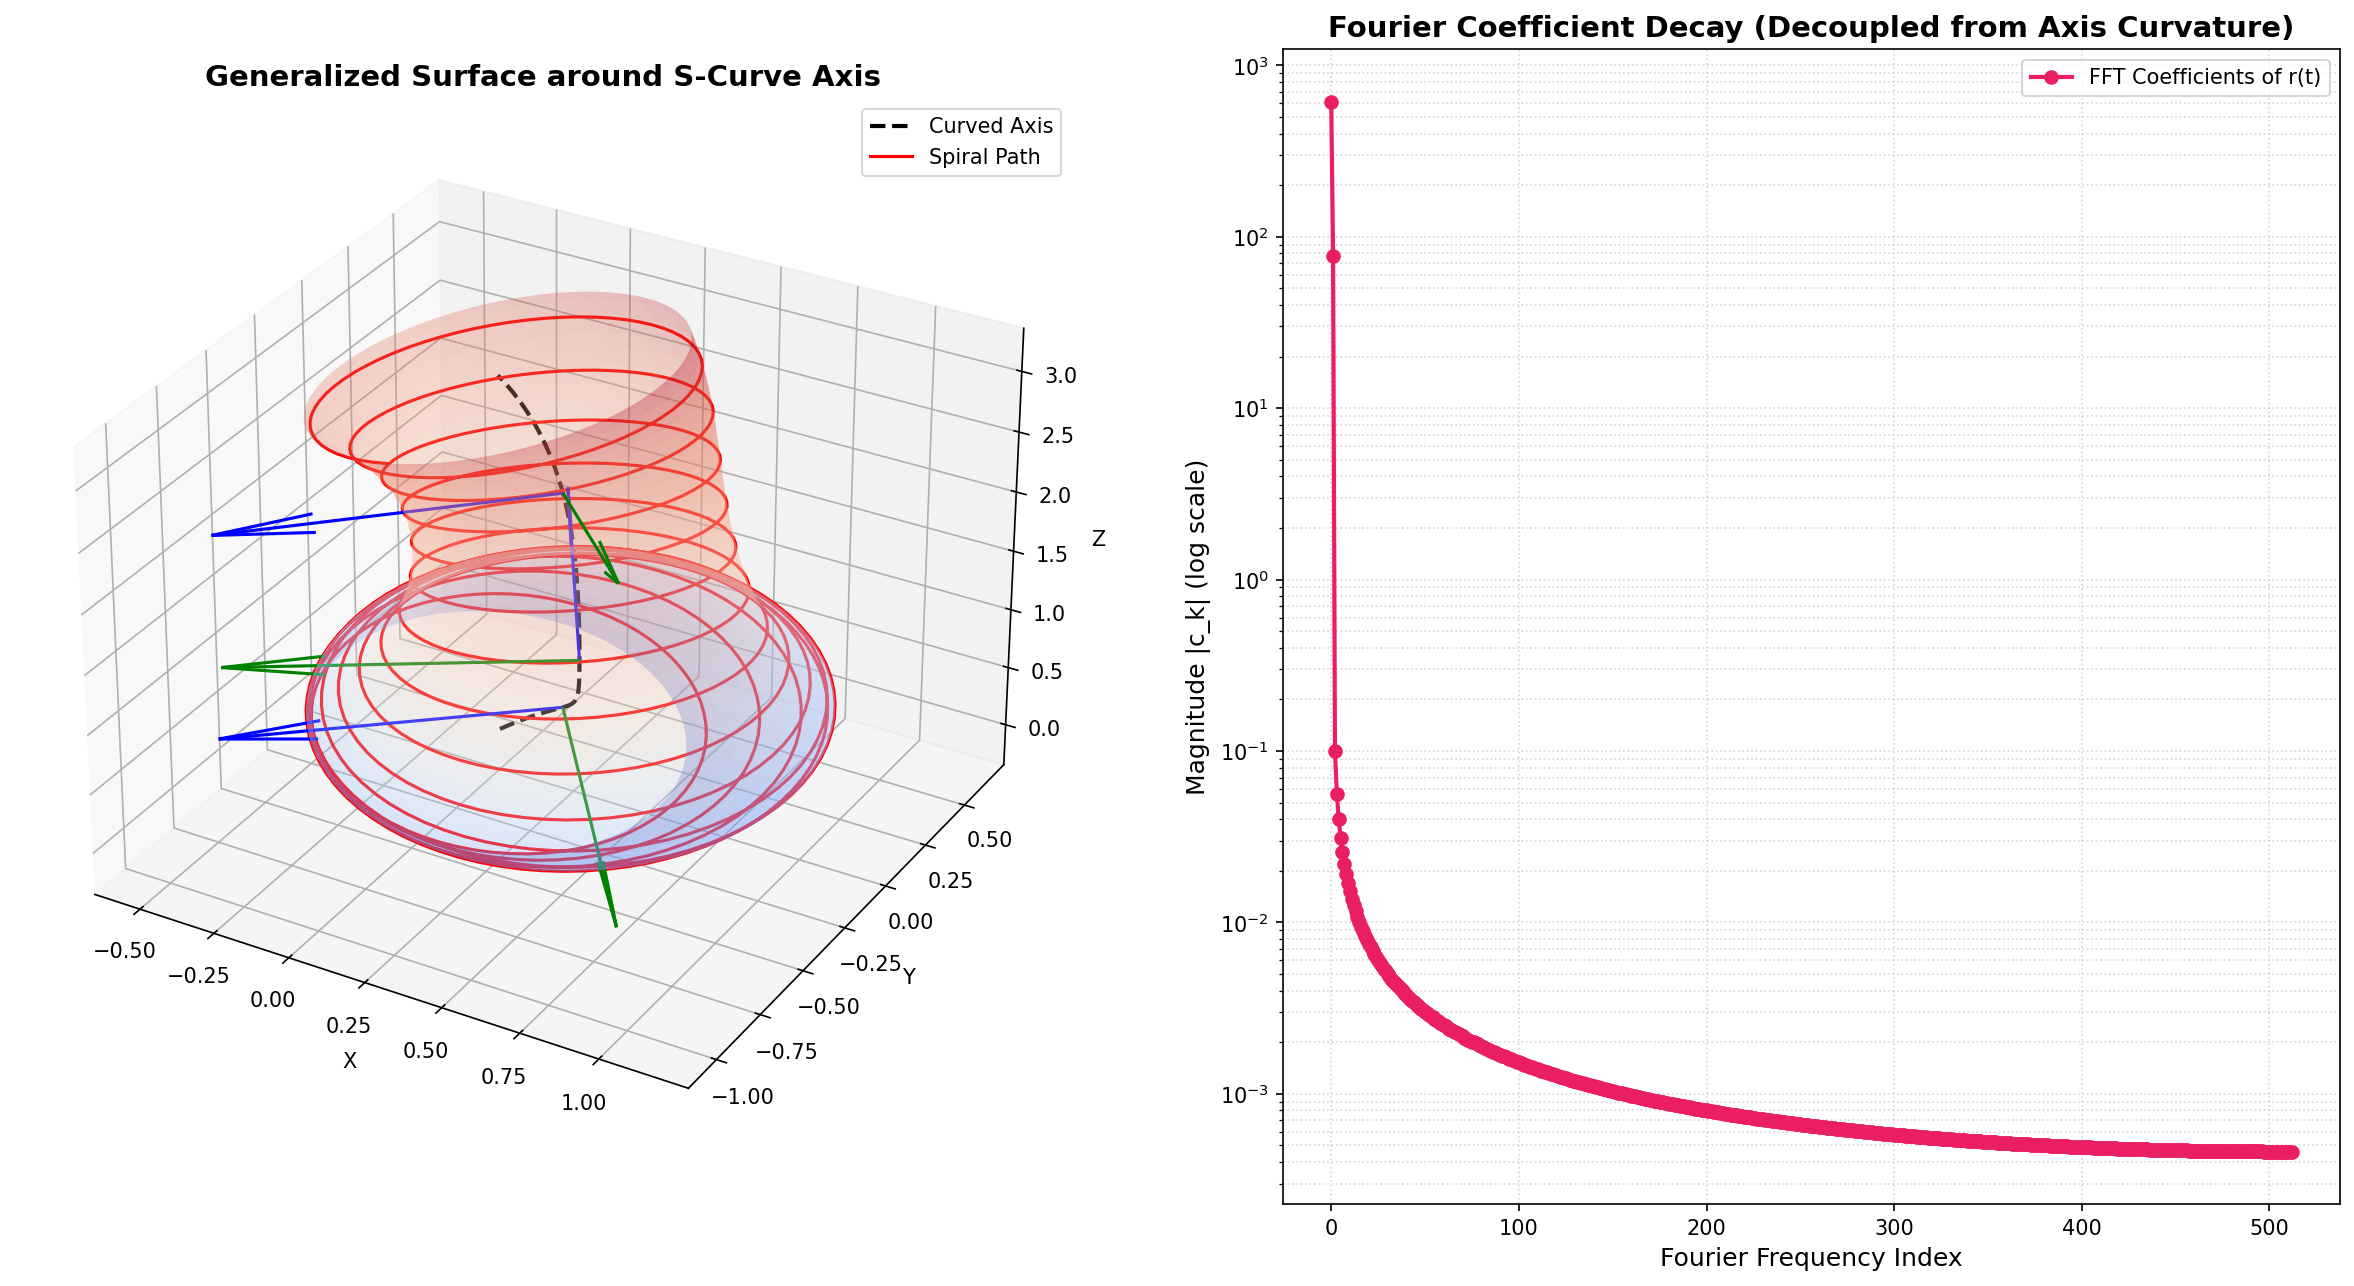
\includegraphics[width=0.95\textwidth]{figures/curved_axis_surface.png}
	\caption{Generalized surface of revolution around a curved S-curve axis (left panel). The local Frenet coordinate frames are shown along the axis. The right panel illustrates the Fourier coefficient decay of the extracted 1D spiral radius signal, demonstrating that curvature does not degrade spectral compressibility when coordinates are defined relative to the local moving frame.}
	\label{fig:curved_axis_surface}
\end{figure}

\section{Quaternionic Parameterization}

\subsection{Unit Quaternions and SU(2)}

Rather than tracking three vectors $(\mathbf{T}, \mathbf{N}, \mathbf{B})$ independently, we encode the entire Frenet frame in a single unit quaternion $q(s) \in \mathbb{H}$, $\|q\| = 1$ \cite{Altmann}.

\begin{definition}[Quaternionic Frame Equation]
	The Frenet--Serret equations are equivalent to the quaternionic differential equation
	\begin{equation}
		\frac{dq}{ds} = \frac{1}{2} q(s) \, \omega(s),
	\end{equation}
	where $\omega(s) = \tau(s)\,\mathbf{i} + \kappa(s)\,\mathbf{k}$ is the pure quaternion encoding the curvature and torsion.
\end{definition}

\subsection{The Sandwich Operator and Quantum Mechanics}

To rotate a 3D vector $\mathbf{v}$ (embedded as the pure quaternion $v = 0 + v_x\mathbf{i} + v_y\mathbf{j} + v_z\mathbf{k}$), we apply:
\begin{equation}
	v' = q \, v \, q^{-1}.
\end{equation}

\begin{remark}[Connection to Quantum Observables]
	This is structurally identical to the quantum mechanical expectation value $\langle \hat{A} \rangle = \langle \psi | \hat{A} | \psi \rangle$. Unit quaternions map to $\operatorname{SU}(2)$ (the double cover of $\operatorname{SO}(3)$), so tracing a path $q(s)$ along the axis curve is equivalent to tracking the continuous unitary evolution of a spin-$\frac{1}{2}$ state. The target curve behaves as an observable whose expectation value evolves along the axis.
\end{remark}

\begin{figure}[htbp]
	\centering
	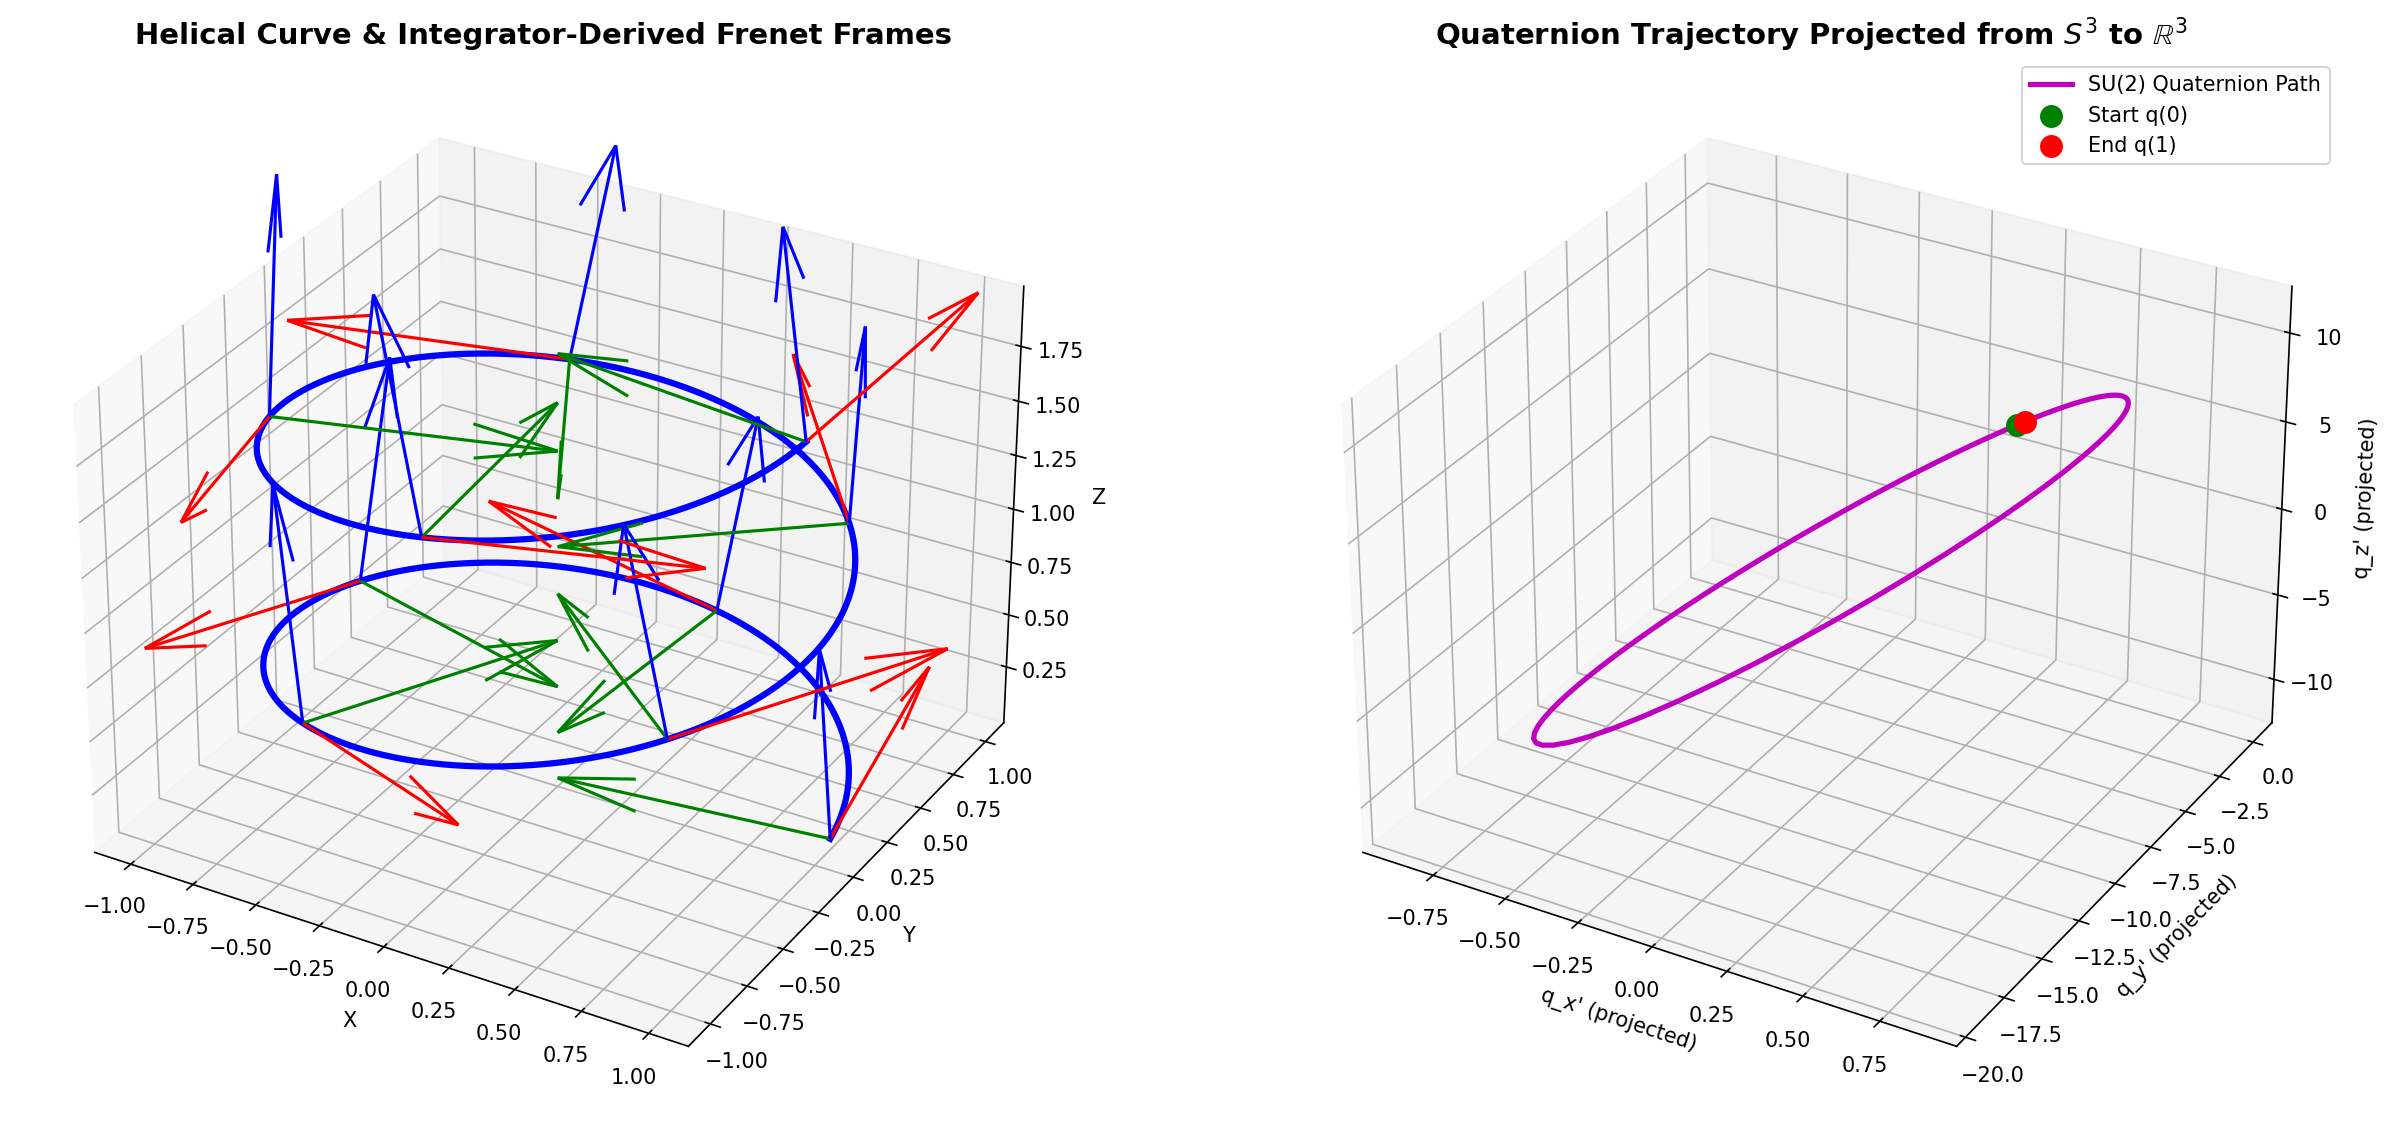
\includegraphics[width=0.95\textwidth]{figures/quaternion_trajectory.png}
	\caption{Quaternionic frame integration along a 3D helical space curve. The left panel shows the 3D curve and the corresponding coordinate frames computed via Runge-Kutta 4th-order integration of $dq/ds = \frac{1}{2}q\omega$. The right panel shows the unit quaternion trajectory $q(s) \in S^3$ projected stereographically into $\mathbb{R}^3$.}
	\label{fig:quaternion_trajectory}
\end{figure}

\section{The Inverse Problem: Unwrapping to a Cylinder}

\subsection{Finding the Straightening Axis}

Given a target curve $C_1(s)$, we ask: \emph{what axis curve $\gamma(s)$ produces a constant radius $r(s) = c$?}

If $r(s) = c$ is constant, then $C_1(s) = \gamma(s) + c \, \mathbf{N}(s)$ is an \emph{offset curve} (or parallel curve) of $\gamma$. The required axis is the \emph{evolute} of $C_1$---the locus of centers of curvature:
\begin{equation}
	\gamma(s) = C_1(s) - \frac{1}{\kappa_{C_1}(s)} \, \mathbf{N}_{C_1}(s).
\end{equation}

\subsection{Application: 3D Model Representation and Compression}

Consider a 3D model (e.g., a human head) represented in cylindrical coordinates $(r, \theta, z)$. Slicing in the $zr$-plane at each angle $\theta$ produces a set of 2D curves $\{C_\theta\}$. For each such slice, solving the inverse problem yields an axis curve $\gamma_\theta$ that ``unwraps'' the complex organic geometry into a cylinder. This is the continuous generalization of Binford's generalized cylinders \cite{Binford}, which Marr and Nishihara \cite{MarrNishihara} proposed as a canonical representation for spatial organization in biological shapes. Chaining this operation across all slices transforms the full 3D surface into a collection of cylinders and smooth residual surfaces.

\begin{remark}[Connection to Offset Curve Convergence]
	This operation is related to a classical result in the geometry of curves: given a convex closed curve, the iterated offset curve (drawn at constant distance in every direction) converges to a circle. Similarly, iterating the ``unwrap to cylinder'' operation successively smooths any convex surface.
\end{remark}

\begin{figure}[htbp]
	\centering
	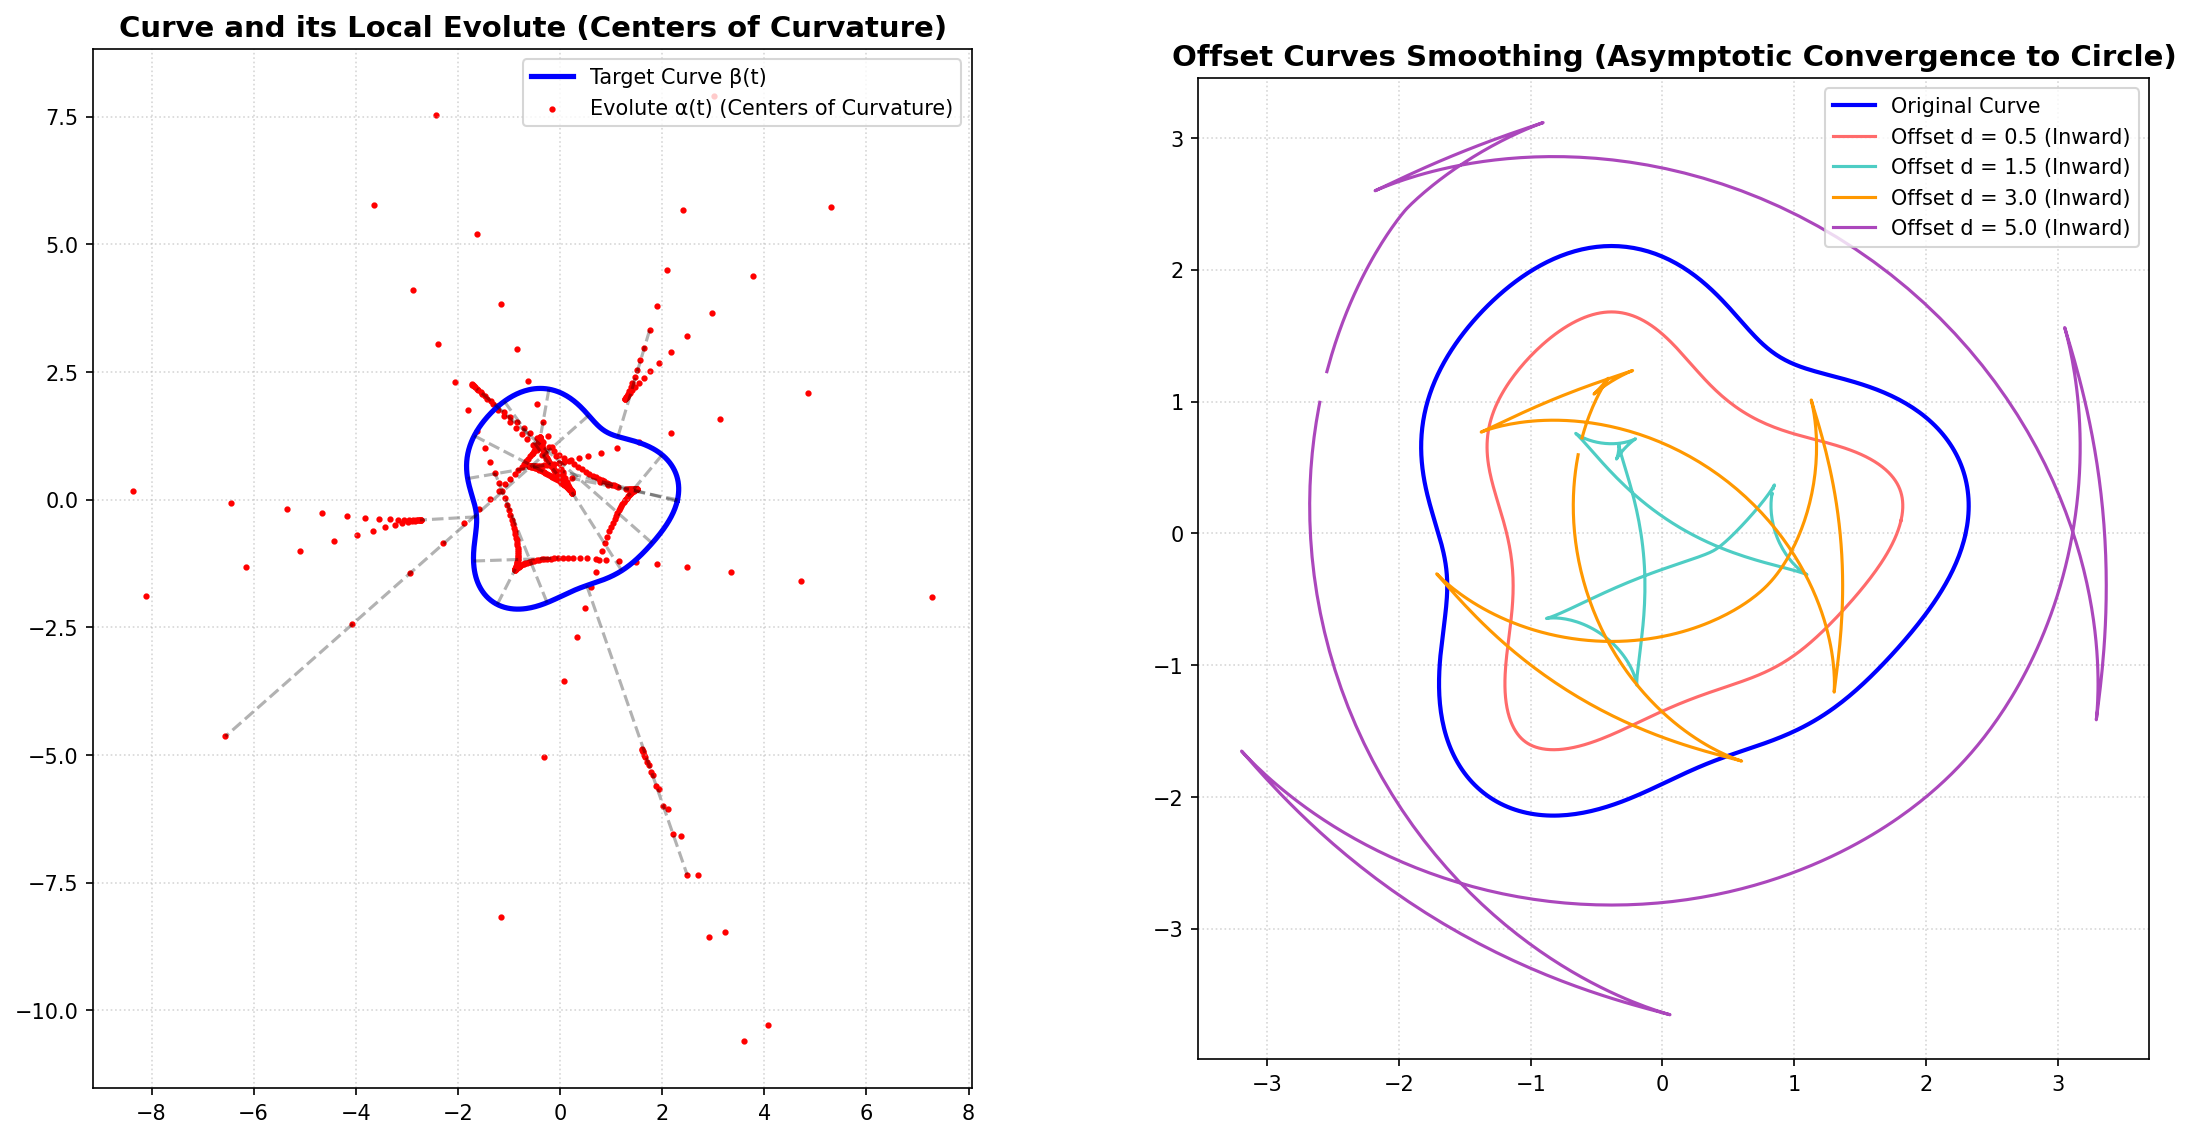
\includegraphics[width=0.95\textwidth]{figures/evolute_smoothing.png}
	\caption{The evolute unwrapping mapping (left panel), showing a wavy target closed curve in blue, its evolute (centers of curvature) in red, and normal projection lines. The right panel shows parallel offset curves at various distances; as the offset distance $d \to \infty$, the curves smooth out and converge asymptotically to perfect circles.}
	\label{fig:evolute_smoothing}
\end{figure}

\section{The Spiral Limit and Dimensional Reduction}

\subsection{From Discrete Wraps to Continuous Surfaces}

Consider a single helical path wrapping around the generalized surface with $n$ periods between the endpoints $a$ and $b$:
\begin{equation}
	\mathbf{c}_n(t) = \gamma(s(t)) + r(s(t))\bigl[\cos(n \cdot 2\pi t) \; \mathbf{N}(s(t)) + \sin(n \cdot 2\pi t) \; \mathbf{B}(s(t))\bigr],
\end{equation}
where $t \in [0, 1]$ and $s(t) = a + (b - a)t$.

At $n = 1$, this is a single loop. As $n$ increases, the spiral wraps tighter and tighter. In the limit $n \to \infty$, the image of $\mathbf{c}_n$ is dense in the surface, analogous to a space-filling curve constrained to a 2D manifold.

\begin{proposition}[Dimensional Reduction]
	The spiral path $\mathbf{c}_n(t)$ reduces the surface to a $1$-dimensional signal: in the limit $n \to \infty$, the image $\operatorname{Im}(\mathbf{c}_n)$ is dense in the generalized surface of revolution $\mathcal{M}$.
\end{proposition}

This density property is a geometric analogue of Kronecker's theorem on torus windings, which forms the core of Weyl's equidistribution theorem \cite{Weyl}.

\begin{proof}
	The surface $\mathcal{M}$ is parameterized by the smooth map $\mathbf{r}(s, \theta) = \gamma(s) + r(s)[\cos\theta \, \mathbf{N}(s) + \sin\theta \, \mathbf{B}(s)]$ over $(s, \theta) \in [a, b] \times \mathbb{R}/2\pi\mathbb{Z}$. Since $[a, b] \times \mathbb{R}/2\pi\mathbb{Z}$ is compact and $\mathbf{r}$ is smooth, $\mathbf{r}$ is Lipschitz continuous.
	
	Let $\mathbf{p} = \mathbf{r}(s_0, \theta_0) \in \mathcal{M}$ be any point on the surface, and let $\epsilon > 0$. We must show that there exists $t \in [0,1]$ such that $\|\mathbf{c}_n(t) - \mathbf{p}\| < \epsilon$ for sufficiently large $n$. By Lipschitz continuity, it suffices to show that we can get arbitrarily close in the parameter space, i.e., there exists $t \in [0,1]$ such that $|s(t) - s_0| < \delta$ and $|2\pi n t - \theta_0| < \delta \pmod{2\pi}$ for a small $\delta > 0$.
	
	Choose the base parameter $t_0 \in [0, 1]$ such that $s(t_0) = s_0$, which gives $t_0 = \frac{s_0 - a}{b - a}$. Now perturb $t_0$ by a small displacement $\Delta t$, setting $t = t_0 + \Delta t$, where we restrict $|\Delta t| < \frac{\delta}{b - a}$ to ensure $|s(t) - s_0| < \delta$. The angular coordinate along the spiral path at $t$ is:
	\begin{equation}
		\theta(t) = 2\pi n t \pmod{2\pi} = 2\pi n t_0 + 2\pi n \Delta t \pmod{2\pi}.
	\end{equation}
	The set of angles accessible under the restriction on $\Delta t$ forms an interval of length $2\pi n \frac{2\delta}{b-a}$. Once the length of this interval exceeds $2\pi$ (which occurs when $n \geq \frac{b-a}{2\delta}$), the image of the interval under the projection modulo $2\pi$ covers the entire circle $[0, 2\pi)$ completely. Thus, for any $n \geq \frac{b-a}{2\delta}$, there exists a perturbation $\Delta t$ satisfying the boundary constraints that maps $\theta(t)$ exactly to $\theta_0 \pmod{2\pi}$. Hence, the spiral path passes within $\epsilon$ of any point on the surface.
\end{proof}

\subsection{Compression via the Spiral Transform}

Sampling the radius $r$ along the spiral path produces a $1$-dimensional waveform $r(t)$.

\begin{itemize}
	\item A perfect cylinder yields $r(t) = \text{const}$: a single Fourier coefficient.
	\item A smooth vase yields a slowly varying $r(t)$: a few low-frequency coefficients suffice.
	\item A detailed organic surface (face, head) yields $r(t)$ with high-frequency ripples at feature locations (nose, eyes), but with strong spatial correlation throughout.
\end{itemize}

Because organic 3D surfaces have immense spatial correlation (the nose blends smoothly into the cheek), the Fourier transform of $r(t)$ concentrates energy in the low-frequency coefficients. High-frequency coefficients decay rapidly and can be discarded with negligible perceptual loss.

\begin{figure}[htbp]
	\centering
	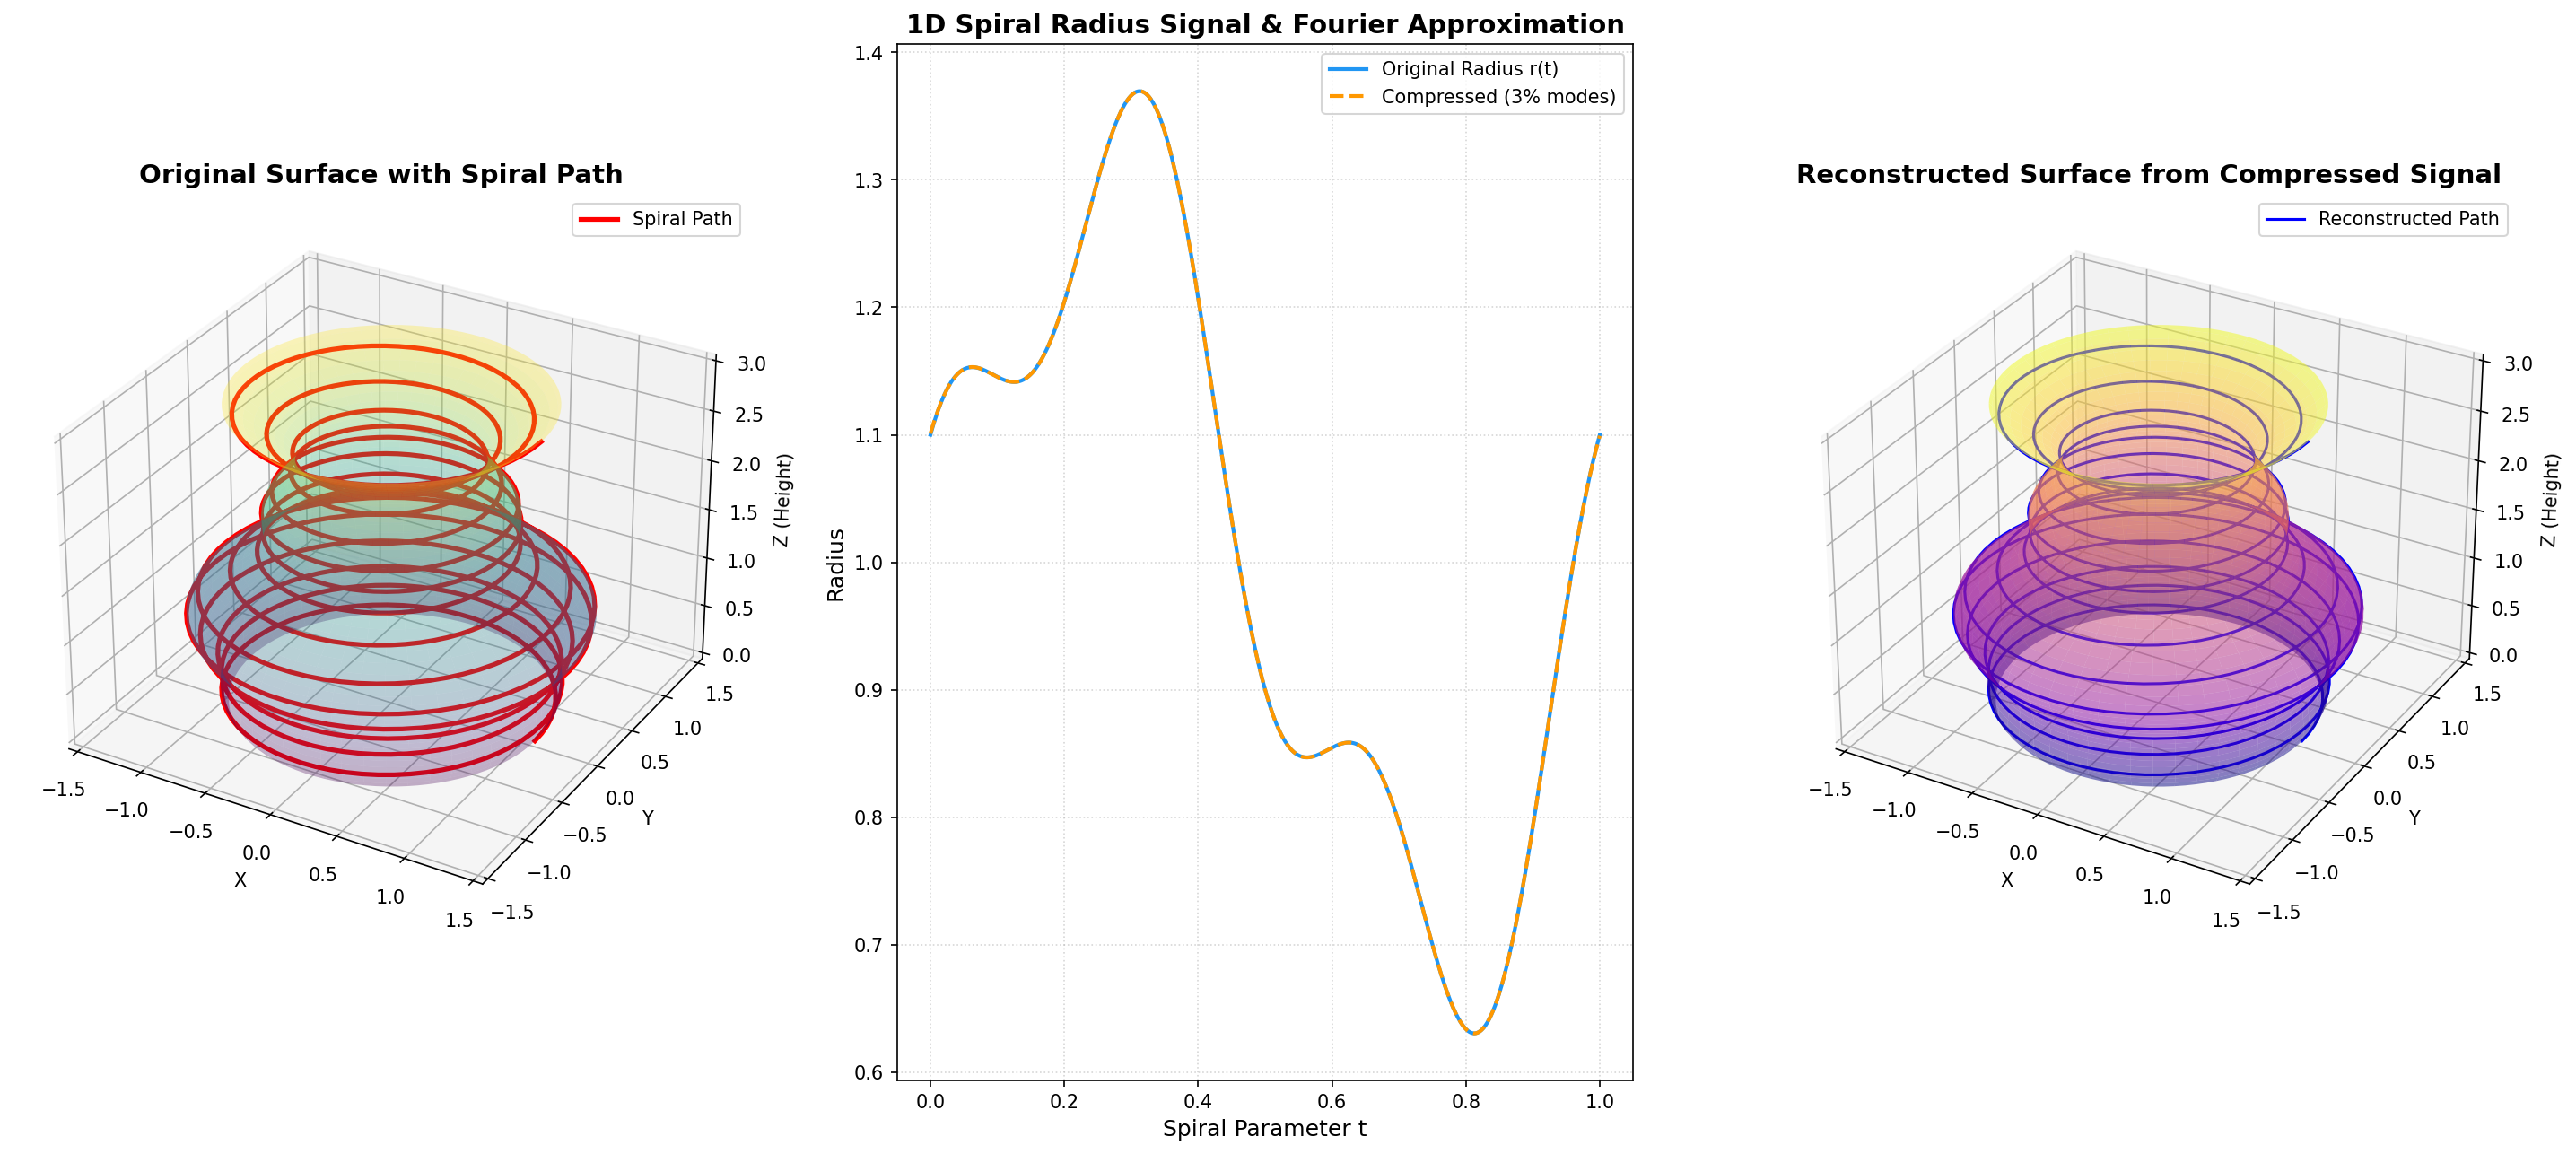
\includegraphics[width=0.95\textwidth]{figures/spiral_transform_reconstruction.png}
	\caption{The 3D spiral transform and surface reconstruction. The left panel shows the original 3D vase surface with the winding spiral path. The middle panel plots the extracted 1D radius signal $r(t)$ and its compressed Fourier reconstruction keeping only the top $3\%$ of modes. The right panel shows the reconstructed 3D surface, demonstrating lossless geometric recovery from a highly compressed spectral representation.}
	\label{fig:spiral_transform_reconstruction}
\end{figure}

\begin{remark}
	This resolves the apparent contradiction with Part~II. Fourier compression fails for \emph{discrete, independent} binary data because the degrees of freedom do not decay spectrally. But for \emph{continuous, correlated} geometric data, the Fourier transform exploits spatial correlation to achieve genuine compression. The spiral transform converts a 3D surface into exactly the type of smooth, correlated signal that Fourier analysis was designed to compress.
\end{remark}

\subsection{Connection to Fourier Analysis on Lie Groups}

Because quaternions are non-commutative ($\mathbf{i}\mathbf{j} \neq \mathbf{j}\mathbf{i}$), the limit of infinitesimal rotations along the axis does not yield a standard Fourier decomposition. Instead, it maps onto the \emph{Spherical Fourier Transform} or Fourier analysis on the Lie group $\operatorname{SU}(2)$.

In this framework, the 3D shape is decomposed not into flat sines and cosines, but into \emph{Wigner $D$-matrices}---the irreducible representations of $\operatorname{SU}(2)$:
\begin{equation}
	f(\alpha, \beta, \gamma) = \sum_{\ell=0}^{\infty} \sum_{m=-\ell}^{\ell} \sum_{m'=-\ell}^{\ell} \hat{f}^{\ell}_{mm'} \, D^{\ell}_{mm'}(\alpha, \beta, \gamma),
\end{equation}
where the Euler angles $(\alpha, \beta, \gamma)$ parameterize the rotation. These are the same spherical harmonics used in quantum mechanics to describe electron orbital angular momentum.

%=============================================================================
\section{Conclusion and Unifying Perspective}
%=============================================================================

The three parts of this paper trace a common arc: the search for the right \emph{representation space} in which structure becomes compressible.

In Part~I, we showed that a binary string's hidden periodicity is invisible to first-order entropy but revealed by block entropy, and that the FFT efficiently identifies the optimal block size---the ``fundamental frequency'' of the data. In Part~II, we proved that embedding discrete data into continuous domains cannot circumvent the conservation of degrees of freedom: information is neither created nor destroyed by a change of basis, and the floating-point overhead inflates the representation. In Part~III, we demonstrated that for data which \emph{already} lives in a continuous, correlated domain (3D geometry), a carefully constructed spiral dimensional reduction---parameterized by quaternionic frames that obey the same algebra as quantum spin---produces exactly the type of smooth, spectrally concentrated signal that Fourier analysis excels at compressing.

The unifying principle is that \emph{compression is possible when and only when the representation captures the correlations of the source}. Block coding captures sequential patterns. Fourier analysis captures smooth spatial correlations. The quaternionic spiral transform captures the rotational symmetry of surfaces. Each tool succeeds precisely in the domain for which it was designed, and fails when applied across that boundary.

\begin{thebibliography}{9}

\bibitem{CoverThomas}
T. M. Cover and J. A. Thomas,
\emph{Elements of Information Theory}, 2nd ed.
Hoboken, NJ: Wiley-Interscience, 2006.

\bibitem{DoCarmo}
M. P. do Carmo,
\emph{Differential Geometry of Curves and Surfaces}, 2nd ed.
Mineola, NY: Dover Publications, 2016.

\bibitem{Altmann}
S. L. Altmann,
\emph{Rotations, Quaternions, and Double Groups}.
Mineola, NY: Dover Publications, 2005.

\bibitem{Weyl}
H. Weyl,
``\"Uber die Gleichverteilung von Zahlen mod. Eins,''
\emph{Mathematische Annalen}, vol. 77, no. 3, pp. 313--352, 1916.

\bibitem{Binford}
T. O. Binford,
``Visual perception by computer,''
in \emph{IEEE Conference on Systems and Control}, Miami, FL, Dec. 1971.

\bibitem{MarrNishihara}
D. Marr and H. K. Nishihara,
``Representation and recognition of the spatial organization of three-dimensional shapes,''
\emph{Proceedings of the Royal Society of London. Series B. Biological Sciences}, vol. 200, no. 1140, pp. 269--294, 1978.

\end{thebibliography}

\end{document}
